\documentclass[11pt,a4paper]{article}
\usepackage{graphicx}
\usepackage{amsmath}
\usepackage{amssymb}
\usepackage{multicol}
\usepackage{tcolorbox}
\usepackage{xcolor}
\usepackage{geometry}
\usepackage{tikz}
\usepackage{array}
\geometry{margin=0.8in}

% Define colors
\definecolor{mlblue}{RGB}{31, 119, 180}
\definecolor{mlorange}{RGB}{255, 127, 14}
\definecolor{mlgreen}{RGB}{44, 160, 44}
\definecolor{mlred}{RGB}{214, 39, 40}
\definecolor{mlpurple}{RGB}{148, 103, 189}

\title{\Large\textbf{Discovery Learning 2: The Feature Detective}\\
\vspace{0.3em}
\normalsize What Makes Things Similar?}
\author{Machine Learning for Smarter Innovation - Pre-Lecture Activity}
\date{}

\begin{document}
\maketitle
\vspace{-1em}

\begin{tcolorbox}[colback=mlgreen!10, colframe=mlgreen!50, title=Learning Objectives]
\small
By completing this activity, you will discover:
\begin{itemize}
\item How different features lead to different groupings
\item Why feature selection is critical for clustering
\item What happens when we have too many features (curse of dimensionality)
\end{itemize}
\end{tcolorbox}

\section*{The Startup Dataset}
You're a venture capitalist analyzing 20 startups. Each has multiple features - but which ones matter for grouping?

\begin{center}
\footnotesize
\renewcommand{\arraystretch}{0.85}
\begin{tabular}{|l|l|c|c|c|c|}
\hline
\textbf{Startup Name} & \textbf{Industry} & \textbf{Employees} & \textbf{Funding (\$M)} & \textbf{Age (yrs)} & \textbf{Growth (\%/yr)} \\
\hline
TechnoAI & AI/ML & 45 & 12.5 & 2 & 150 \\
GreenLeaf & CleanTech & 28 & 5.2 & 3 & 85 \\
DataFlow & Analytics & 67 & 22.0 & 5 & 110 \\
HealthHub & HealthTech & 34 & 8.7 & 2 & 125 \\
EduSmart & EdTech & 23 & 3.5 & 1 & 200 \\
FinanceForward & FinTech & 89 & 45.0 & 6 & 95 \\
CloudNine & Cloud & 56 & 18.0 & 4 & 105 \\
BioGenix & BioTech & 42 & 15.0 & 3 & 90 \\
CyberShield & Security & 38 & 9.8 & 2 & 140 \\
MarketMind & MarTech & 19 & 2.1 & 1 & 175 \\
RoboWorks & Robotics & 51 & 20.0 & 4 & 100 \\
SocialSphere & Social Media & 72 & 28.0 & 5 & 80 \\
GameOn & Gaming & 41 & 11.0 & 3 & 120 \\
FoodTech Plus & FoodTech & 26 & 4.5 & 2 & 135 \\
AutoDrive & Autonomous & 63 & 35.0 & 5 & 88 \\
VirtualSpace & VR/AR & 31 & 7.2 & 2 & 155 \\
LogisticsPro & Logistics & 47 & 13.5 & 4 & 98 \\
AgriTech Now & AgTech & 22 & 3.0 & 1 & 180 \\
RetailRevolution & E-commerce & 58 & 24.0 & 6 & 75 \\
BlockChainBase & Blockchain & 36 & 10.0 & 3 & 115 \\
\hline
\end{tabular}
\end{center}

\section*{Exercise 1: Single Feature Clustering}

\subsection*{Task A: Cluster by Industry Only}
Group the startups into 3 clusters based ONLY on their industry type. Write the startup names in each cluster:

\begin{center}
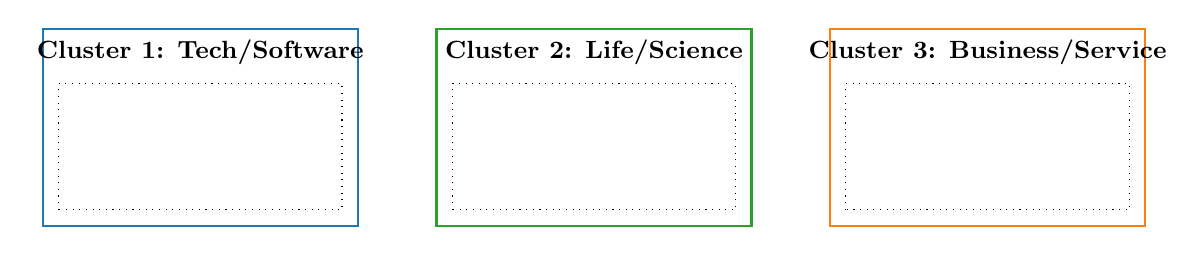
\begin{tikzpicture}
\draw[thick, mlblue] (0,0) rectangle (4,2.5);
\node[font=\small] at (2,2.2) {\textbf{Cluster 1: Tech/Software}};
\draw[dotted] (0.2,0.2) rectangle (3.8,1.8);

\draw[thick, mlgreen] (5,0) rectangle (9,2.5);
\node[font=\small] at (7,2.2) {\textbf{Cluster 2: Life/Science}};
\draw[dotted] (5.2,0.2) rectangle (8.8,1.8);

\draw[thick, mlorange] (10,0) rectangle (14,2.5);
\node[font=\small] at (12,2.2) {\textbf{Cluster 3: Business/Service}};
\draw[dotted] (10.2,0.2) rectangle (13.8,1.8);
\end{tikzpicture}
\end{center}

\subsection*{Task B: Cluster by Funding Only}
Now group the SAME startups into 3 clusters based ONLY on funding amount:
\begin{itemize}
\item Low funding: < \$10M
\item Medium funding: \$10M - \$25M  
\item High funding: > \$25M
\end{itemize}

\begin{center}
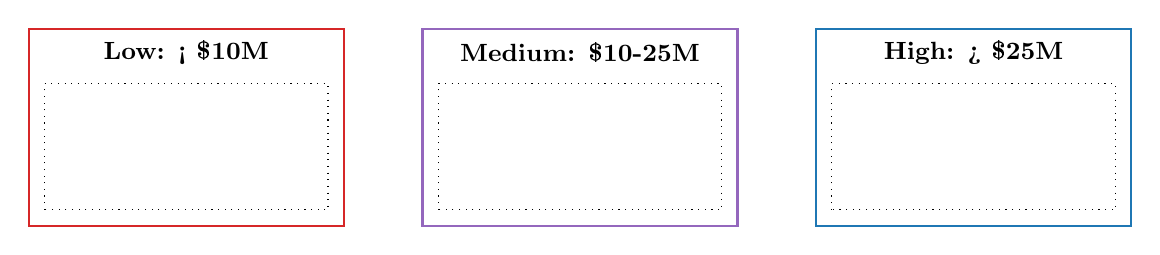
\begin{tikzpicture}
\draw[thick, mlred] (0,0) rectangle (4,2.5);
\node[font=\small] at (2,2.2) {\textbf{Low: < \$10M}};
\draw[dotted] (0.2,0.2) rectangle (3.8,1.8);

\draw[thick, mlpurple] (5,0) rectangle (9,2.5);
\node[font=\small] at (7,2.2) {\textbf{Medium: \$10-25M}};
\draw[dotted] (5.2,0.2) rectangle (8.8,1.8);

\draw[thick, mlblue] (10,0) rectangle (14,2.5);
\node[font=\small] at (12,2.2) {\textbf{High: > \$25M}};
\draw[dotted] (10.2,0.2) rectangle (13.8,1.8);
\end{tikzpicture}
\end{center}

\begin{tcolorbox}[colback=mlorange!10, colframe=mlorange!50, title=Discovery Question 1]
\textbf{Did the same companies end up together in both clustering approaches?}\\
Give an example of two companies that were together in Task A but separated in Task B:\\
\vspace{0.3em}
Company 1: \underline{\hspace{3cm}} Company 2: \underline{\hspace{3cm}}\\
Why did this happen? \underline{\hspace{8cm}}
\end{tcolorbox}

\newpage

\section*{Exercise 2: Multi-Feature Clustering}

\subsection*{Task C: Your Choice - Combine Features}
Create your own 3 clusters using ANY combination of features. Plot on the grid below:

\begin{center}
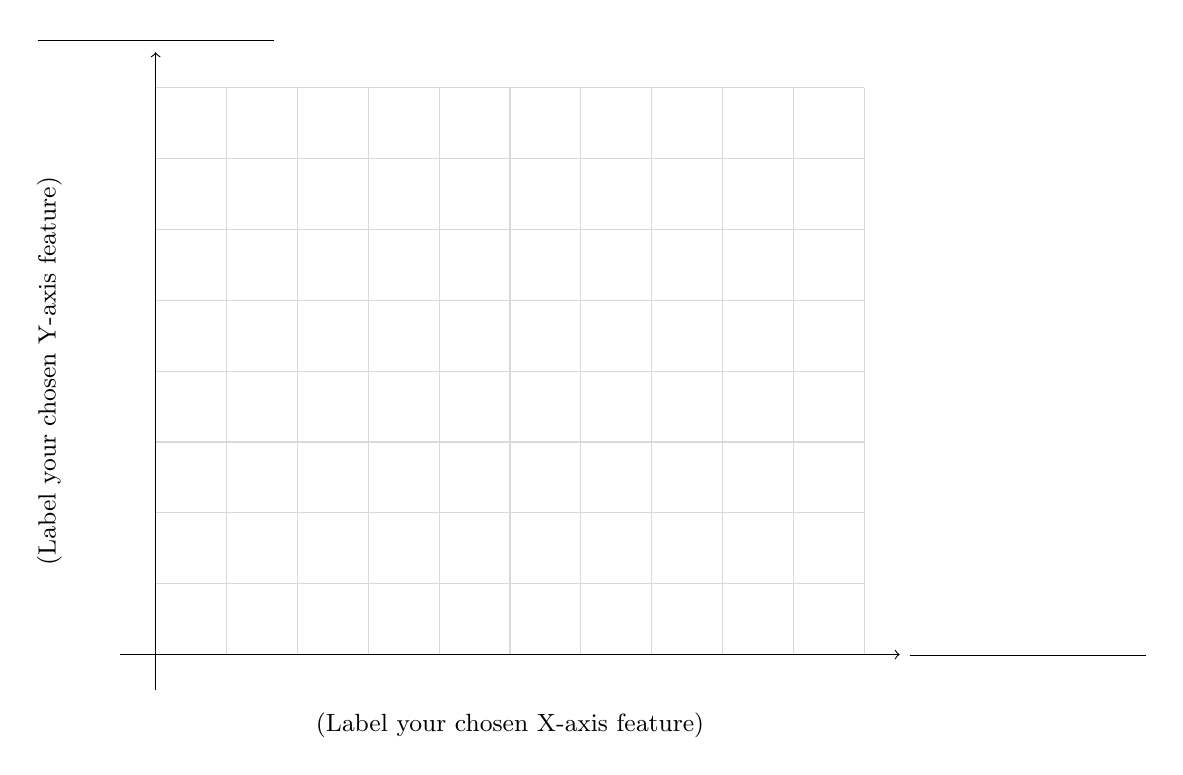
\begin{tikzpicture}[scale=0.9]
% Grid
\draw[gray!30, thin] (0,0) grid (10,8);
% Axes
\draw[->] (-0.5,0) -- (10.5,0) node[right] {\underline{\hspace{3cm}}};
\draw[->] (0,-0.5) -- (0,8.5) node[above] {\underline{\hspace{3cm}}};
\node[font=\small] at (5,-1) {(Label your chosen X-axis feature)};
\node[font=\small, rotate=90] at (-1.5,4) {(Label your chosen Y-axis feature)};
\end{tikzpicture}
\end{center}

\textbf{My clustering criteria:} \underline{\hspace{10cm}}

\section*{Exercise 3: The Curse of Dimensionality}

\subsection*{Task D: Feature Overload}
Imagine adding 5 more features to each startup:
\begin{itemize}
\item Customer satisfaction score (1-10)
\item Office locations (1-20)
\item Product lines (1-50)
\item Patents filed (0-100)
\item Social media followers (100-1M)
\end{itemize}

\begin{center}
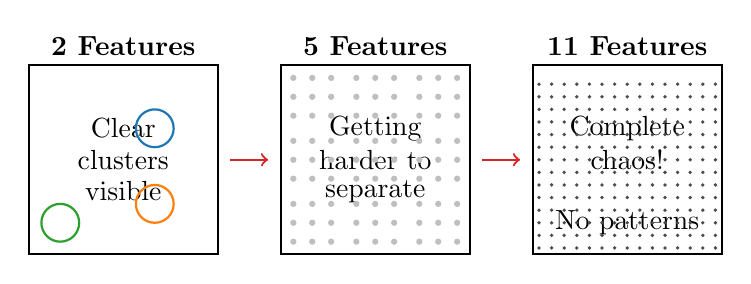
\begin{tikzpicture}[scale=0.8]
% 2D visualization
\draw[thick] (0,0) rectangle (3,3);
\node at (1.5,3.3) {\textbf{2 Features}};
\node at (1.5,2) {Clear};
\node at (1.5,1.5) {clusters};
\node at (1.5,1) {visible};
\draw[mlgreen, thick] (0.5,0.5) circle (0.3);
\draw[mlblue, thick] (2,2) circle (0.3);
\draw[mlorange, thick] (2,0.8) circle (0.3);

% 5D visualization
\draw[thick] (4,0) rectangle (7,3);
\node at (5.5,3.3) {\textbf{5 Features}};
\node at (5.5,2) {Getting};
\node at (5.5,1.5) {harder to};
\node at (5.5,1) {separate};
\foreach \x in {0.2,0.5,0.8,1.2,1.5,1.8,2.2,2.5,2.8}
    \foreach \y in {0.2,0.5,0.8,1.2,1.5,1.8,2.2,2.5,2.8}
        \fill[gray!50] (4+\x,\y) circle (0.05);

% 11D visualization  
\draw[thick] (8,0) rectangle (11,3);
\node at (9.5,3.3) {\textbf{11 Features}};
\node at (9.5,2) {Complete};
\node at (9.5,1.5) {chaos!};
\node at (9.5,0.5) {No patterns};
\foreach \x in {0.1,0.3,0.5,0.7,0.9,1.1,1.3,1.5,1.7,1.9,2.1,2.3,2.5,2.7,2.9}
    \foreach \y in {0.1,0.3,0.5,0.7,0.9,1.1,1.3,1.5,1.7,1.9,2.1,2.3,2.5,2.7}
        \fill[black!70] (8+\x,\y) circle (0.03);

\draw[->, thick, mlred] (3.2,1.5) -- (3.8,1.5);
\draw[->, thick, mlred] (7.2,1.5) -- (7.8,1.5);
\end{tikzpicture}
\end{center}

\begin{tcolorbox}[colback=mlred!10, colframe=mlred!50, title=The Curse of Dimensionality]
As we add more features, the ``distance'' between any two startups becomes less meaningful. 
With 11 features, every startup seems equally far from every other startup!
\end{tcolorbox}

\subsection*{Reflection: Feature Importance Ranking}
If you could only use 3 features to cluster startups for investment decisions, which would you choose?

\begin{center}
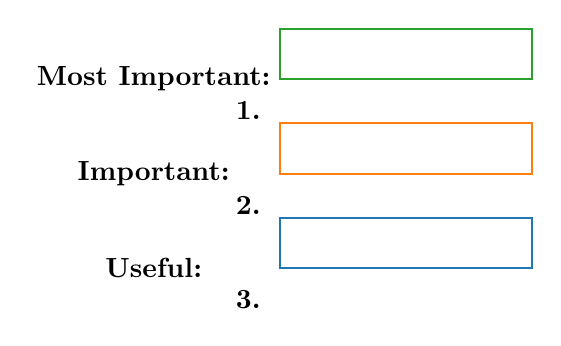
\begin{tikzpicture}[scale=0.8]
\node at (0,0) {\textbf{Most Important:}};
\draw[mlgreen, thick] (2,0) rectangle (6,0.8);
\node at (1.5,-0.5) {\textbf{1.}};

\node at (0,-1.5) {\textbf{Important:}};
\draw[mlorange, thick] (2,-1.5) rectangle (6,-0.7);
\node at (1.5,-2) {\textbf{2.}};

\node at (0,-3) {\textbf{Useful:}};
\draw[mlblue, thick] (2,-3) rectangle (6,-2.2);
\node at (1.5,-3.5) {\textbf{3.}};
\end{tikzpicture}
\end{center}

\textbf{Why these three?} \underline{\hspace{10cm}}\\
\underline{\hspace{14cm}}

\section*{Final Discovery Questions}

\begin{enumerate}
\item \textbf{Pattern Recognition:} Looking at your different clusterings, which feature created the most meaningful groups? Why?\\
\vspace{0.3em}
\underline{\hspace{14cm}}\\
\underline{\hspace{14cm}}

\item \textbf{Scale Challenge:} With 20 startups and 6 features, you could manage this manually. What about 10,000 startups with 50 features each?\\
\vspace{0.3em}
\underline{\hspace{14cm}}\\
\underline{\hspace{14cm}}

\item \textbf{Missing Data:} What if some startups didn't report all features (e.g., private funding amounts)? How would this affect clustering?\\
\vspace{0.3em}
\underline{\hspace{14cm}}\\
\underline{\hspace{14cm}}
\end{enumerate}

\begin{tcolorbox}[colback=mlpurple!10, colframe=mlpurple!50, title=Prepare for Next Class]
You've discovered that clustering depends entirely on which features we choose and how we weight them. 
In our next lecture, you'll learn how machine learning algorithms can:
\begin{itemize}
\item Automatically find the most important features
\item Handle hundreds of dimensions
\item Discover patterns humans would never see
\end{itemize}
Think about: How would you teach a computer to decide which features matter most?
\end{tcolorbox}

\end{document}